\documentclass[12pt]{article}

\usepackage[a4paper,margin=1.5in]{geometry}
\usepackage[strict]{changepage}
\usepackage[scale=0.92]{tgschola}
\usepackage{fouriernc}
\usepackage[T1]{fontenc}

\usepackage{booktabs, threeparttable, adjustbox, tabularx, longtable}
\usepackage{amsmath, amssymb, amsthm, bbm}
\usepackage{hyperref, achicago}
\usepackage{caption, graphicx}
\usepackage{secdot, sectsty}
\usepackage{pdflscape}
\usepackage{placeins}
\usepackage{xcolor}

\fontfamily{qcs}
\linespread{1.1}
\urlstyle{tt}

\allsectionsfont{\rmfamily}
\sectionfont{\normalsize}
\subsectionfont{\normalfont\normalsize\selectfont\itshape}
\subsubsectionfont{\normalfont\normalsize\selectfont\itshape}

\sectiondot{subsection}

\renewcommand\thesection{\Roman{section}}
\renewcommand\thesubsection{\thesection.\Alph{subsection}}
\renewcommand\thesubsubsection{\thesubsection.\arabic{subsubsection}}

\newcommand{\specialcell}[2][c]{\begin{tabular}[#1]{@{}c@{}}#2\end{tabular}}
\renewcommand{\today}{\ifcase \month \or January\or February\or March\or April\or May \or June\or July\or August\or September\or October\or November\or December\fi~ \number \year}

\begin{document}

\title{\textsc{Using Lotteries to Encourage Saving: Experimental Evidence from Kenya}\protect\footnote{We are grateful to the study participants for generously giving their time. We thank Jonathan Page and Arun Varghese for excellent research assistance. This study was pre-registered with the AEA RCT registry (AEARCTR-0000893). Files for replication are available at \url{https://github.com/princetonbpl/akiba-lottery-pub}.}}

\author{Justin Abraham\thanks{Department of Economics. University of California, San Diego. \protect\href{mailto:jabraham@ucsd.edu}{\nolinkurl{jabraham@ucsd.edu}}.}, Merve Akbas\thanks{Department of Economics. Duke University. \protect\href{mailto:merve.akbas@duke.edu}{\nolinkurl{merve.akbas@duke.edu}}.}, Dan Ariely\thanks{Fuqua School of Business. Duke University. \protect\href{mailto:dan@danariely.com}{\nolinkurl{dan@danariely.com}}.}, and Chaning Jang\thanks{The Busara Center for Behavioral Economics. \protect\href{mailto:chaning.jang@busaracenter.org}{\nolinkurl{chaning.jang@busaracenter.org}}.}}

\maketitle

	\begin{abstract}

		We evaluate the provision of prize-linked savings accounts (PLS)---savings products that incorporate stochastic returns to deposits---against a standard, interest-bearing deposit account. We provided a PLS product to 311 informal residents in Nairobi, Kenya and observe account activity over a 60-day period. We found that participants with PLS made 42\% more deposits on average over the project period than participants who received a fixed matching incentive of equal expected value. We do not observe any effects due to the lottery incentive on amount deposited over the project period. We show that when presented with potential winnings from previous days, participants with PLS increased gambling activity by 15\%. Our results suggest that the PLS is a promising tool to improve savings among the poor and that product design has considerable implications for gambling behavior.

		% add time-dependent results and ROSCA savings results
        % add hypothesis and supporting evidence.

		\medskip \noindent
		\textbf{JEL Classification}: D14, E21, G11

	\end{abstract}

\newpage

\section{Introduction}

	Saving is one of the most important avenues toward economic development; it provides a means to smooth disastrous shocks and the ability to make profitable investments. There exists, however, a host of obstacles that prevent poor households from accruing savings to their advantage. In the absence of effective and affordable savings technologies, savings are susceptible to extraction by theft or by social claimants \shortcite{banerjee_economic_2007,schaner_cost_2011}. Poor households often resort to methods of saving that can be costly and have limited functionality \shortcite{collins_portfolios_2009,karlan_savings_2014}. Policies that expand access to financial services have successfully increased account ownership but have been less effective at encouraging usage \shortcite{dupas_why_2013,karlan_banking_2016}. In Kenya, 27.5\% of low income households own an account yet 9.9\% save with a financial institution \shortcite{demirguc-kunt_global_2015}.

	On the demand side, knowledge gaps, mistrust of financial institutions, and behavioral biases prevent the poor from saving as much as they would like. Product designs that target behavioral barriers have been shown to be extremely cost-effective, especially compared to direct  subsidies.\footnote{\shortciteN{karlan_price_2018} estimate very low interest rate elasticities and limited impacts of easing account ownership requirements. \shortciteN{schaner_persistent_nodate} boost short-run individual savings by USD 1.38 with rates of up to 20\%.} Track-keeping objects \shortcite{akbas_how_2016}, SMS reminders \shortcite{karlan_getting_2010}, and default contributions \shortcite{thaler_save_2004,chetty_active_2014} address undersaving due to limited attention. Binding commitment devices, in the form of account restrictions \shortcite{ashraf_tying_2006} or the application of social pressure \shortcite{dupas_why_2013}, can help individuals with time-inconsistent behavior follow through on saving.

	Our study asks how savings products can leverage consumers' risk attitudes to influence savings behavior. We examine the effects of prize-linked savings (PLS) accounts, a product that incorporates lottery-like payoffs to traditional savings accounts. Savers using PLS accounts receive a probabilistic payoff in addition to, or foregoing regular interest. Common among most PLS products is that consumers face no risk of negative returns. Lottery expenditures demonstrate an inverse relationship with socioeconomic status, which suggests that poor households may be especially responsive to lottery-like incentive structures \shortcite{brown_socio-economic_1992,barnes_gambling_2011}. Furthermore, there is some evidence that usage of lottery-linked accounts displaces costly gambling behavior \shortcite{cookson_when_2016}. Such findings make the product a potentially attractive tool for promoting financial inclusion.

	% The demand for PLS and for gambling in general coupled with risk-averse behavior (e.g. seeking insurance) is well-documented

	PLS have been in use since at least the 17\textsuperscript{th} century and presently exist in various forms around the globe \shortcite{murphy_lotteries_2005,kearney_making_2010}. NS\&I Premium Bonds in the U.K., First National Bank's ``A-Million-A-Month'' Account in South Africa and Individual Development Accounts (IDAs) in the United States are some prominent examples of this type of savings product.

    % Recently legal in the US, more recent examples

	The present study is a laboratory and field experiment analyzing the effects of PLS on savings behavior. We provided a mobile savings product to 311 informal residents in Nairobi, Kenya and observed account activity over a 60-day period. We minimized transactions costs to saving by utilizing Safaricom's Sambaza mobile savings technology. This platform allowed us to collect detailed data on participant transactions and to examine savings behavior over time. Roughy one-third of our sample was randomly assigned a savings account which provided a fixed 5\% match daily to desposits made that day. A second group was assigned an account that yielded stochastic returns equal in expectation to the 5\% match through a lottery conducted on a daily basis. For each day a participant makes a non-zero deposit, they received a lottery ticket and an opportunity to win a prize instead of the fixed match. We compared the match and lottery groups to determine how PLS impact savings behavior. A third group received the same lottery-linked account with the additional feature that participants received a lottery ticket and observed the lottery results every day regardless of saving. We tested this treatment aginst the lottery treatment to determine whether feedback from lottery results affects decisions to save.

	% Literature on regret aversion in motivating behavior (Machina paradox)
	% Unclear that its regret aversion driving effects (could be biases in subjective probability)

	We found that participants using PLS with feedback made 42\% more deposits on average over the project period than participants receiving the matched incentive. Moreover, this increase in account activity is due to participants making more deposits per day in order to enter the lottery. There were no significant differences in effects on saving between the regular PLS and the PLS with feedback. Interestingly, we find no effect of PLS on total amount saved or on the size of each deposit. Participants made smaller, more frequent deposits compared to the control group. We find no evidence of the PLS displacing savings from other sources. On gambling behavior, we find that participants who used the PLS with feedback reported higher gambling activity 15 percentage points more than the control group.

	% results consistent when modelled at the day level
	% no evidence of decreasing effect over time
	% no evidence of recency effects

	This study contributes to the literature as one of the first randomized evaluations examining the impact of PLS on saving behavior. Moreover, the study's unique experimental design allows us to identify dynamic effects: participants make more frequent deposits to their accounts when given lottery-based returns. This result suggests that a non-pecuniary appeal of gambling, unrelated to prize amounts, may be enough to induce a change in savings behavior. PLS may thus improve utilization among existing account holders and be able to attract new savers to open formal savings accounts. Frequent deposits may also have long-term benefits by encouraging the formation of a savings habit \shortcite{alessie_saving_2009}. From a policy perspective, PLS may not be revenue neutral compared to matching if financial institutions incur greater transaction costs as a result of more frequent deposits.

	% not one of the first, but extends the literature
	% argue that usage is still an important outcome for policy
	% effect on ROSCA participation
	% het effects on savings
	% brune's point about temporary vs persistent preferences implications for policy
	% I will list three characteristics: (1) the importance of the question and of the main results; (2) the  clarity,  organization,  and  length  of  the  paper;  and  (3) its degree of novelty in either method or data.

	Our study also shows that participants with PLS with feedback increased self-reported gambling activity relative to the control group. If PLS contribute to problem gambling, the program is potentially welfare-decreasing for households susceptible to problem gambling. \shortciteN{cookson_when_2016} reports a 15\% reduction of casino gambling in Nebraska as a result of enrollment in an PLS bundled with an anti-gambling advertising campaign. The difference from our results suggests that additional program components could diminish effects on outside gambling. Overall, we document several advantages of PLS over fixed-incentive schemes when it comes to promoting financial inclusion and show that product design is crucial in moderating adverse effects on gambling behavior.

	% het effects on gambling

	The remainder of the paper is structured as follows. Section \ref{sec:litreview} presents a brief review of related literature, Section \ref{sec:design} describes our experimental design, Section \ref{sec:est} outlines our estimation strategy, Section \ref{sec:results} discusses our main results, and Section \ref{sec:conclusion} concludes.

\section{Related Literature} \label{sec:litreview}

	How might lotteries induce savings? Preferences for skewed returns are well-documented, so the use of lottery-like structures may play a viable role in incentivizing savings. Models departing from expected utility theory incorporate the overweighting of small probabilities \shortcite{kahneman_advances_1992} and attention to salient payoffs \shortcite{bordalo_salience_2012} in order to account for seemingly risk-loving behavior among risk-averse individuals. Research on preferences for skewness have produced a litany of potential explanations for this phenomenon.\footnote{This paper does not test against these competing explanations and introduces them as a framework for interpreting results.} One broad strand of the literature understands the overweighting of long-odds as a result of persistent preferences for such gambles. Playing the lottery may provide excitement from taking risks and a chance to win a large payoff \shortcite{conlisk_utility_1993}. Similarly, aversion to anticipated regret from foregoing a big prize could drive gambling behavior \shortcite{loomes_regret_1982,zeelenberg_consequences_2004}. Credit-constrained households may also rely on lotteries to save for large, indivisible expenditures \shortcite{kwang_why_1965,herskowitz_gambling_2016}. Alternatively, preferences for gambling may result from bias in subjective probabilities vis-\`{a}-vis true probabilities. The biased weighting of probabilities implies more fickle gambling behavior that depend on exposure to information and repeated choice \shortcite{hertwig_descriptionexperience_2009}.

	% two types: biases in subjective probabilities or preference for skewness
		% bias hypothesis predicts that people can learn over time "debiasing"
		% preference hypothesis predicts no learning
	% explain and elaborate hot-hand and gambler's fallacy
	% Extensive research has tried to explain the higher demand for lotteries and gambling among people with lower income. One approach allows individuals to use subjective probability weighting to over-weight low probability events, e.g. rank-dependent expected utility theory (Quiggin, 1982); cumulative prospect theory (Tversky and Kahneman, 1992). Another approach, skewness, allows utility to depend upon both absolute and relative wealth so that lotteries offer an opportunity to move up in terms of relative wealth (Shefrin and Statman, 2000). Crossley et al. (2011) suggest that people can use lotteries to convexify their budget sets.
	% what is the link to regret aversion? the first point has to do with risk attitudes the second point has to do with violations of independence
	%  The Probability Weighting Function (Drazen Prelec )
	% check lit review in the notes section
	% bilal zia paper on debiasing

	Literature on the demand for PLS is extensive, but evidence of a causal effect on savings behavior is limited. Two recent experimental studies provide evidence of a positive effect of stochastic returns on saving for the future. \shortciteN{atalay_savings_2014} conducted an online portfolio-choice experiment that resulted in participants saving an additional 12 percentage points more with lottery-linked and regular savings than with regular savings alone. Notably, participants who saw an increase in total savings shifted away from lottery expenditures and consumption rather than from regular savings. \shortciteN{filiz-ozbay_lottery_2015} found participants are more likely to delay payments with lottery-like returns compared to guaranteed interest of equivalent expected value. This finding suggests that lottery-linked schemes can be designed to be revenue neutral in expectation for account providers while still promoting savings. Outside the laboratory, evidence surrounding PLS is more limited and diverges somewhat from those findings. \shortciteN{loibl_testing_2016} conducted a randomized evaluation of IDAs in the U.S. that incorporated a lottery-based savings match. That study found no significant effect of the program relative to guaranteed matching, even when it was bundled with reminder calls and frequent deposit deadlines. They attribute the result to liquidity constraints among their sample, which potentially precluded the benefits of behavioral interventions. Lottery-based incentives applied in other domains, including labor supply \shortcite{brune_effect_2015} and health-related behaviors \shortcite{kimmel_randomized_2012,bjorkman_nyqvist_using_2015}, are found to have significant effects.

	% check out brune literature review for empirical evidence in labor, medicine, etc.
	% check out new work by gertler and zia on this
	% Discuss \shortcite{dizon_leveraging_2016}
	% is it reasonable to assume banks are risk neutral?
	% should check whether different results are being driven by regret aversion (would people have been aware that others were winning?)
	% where should we state our priors?
	% regret aversion + CPT = regret affects the reference point https://voxeu.org/article/regret-and-economic-decision-making

	% While we do not detect statistically significant differences in deposits between the \textsc{Lottery} and \textsc{Regret} groups, our estimates point to the importance of regret aversion in supplementing the choice to play by saving. Regret aversion will motivate making deposits if our participants anticipated feeling ``loser regret'' from information that they could have won had they played \shortcite{filiz-ozbay_lottery_2015}. This conforms to suggestive evidence from a cross-sectional study of Dutch lotteries that anticipated regret from winning but not playing relates to future decisions to enter the lottery \shortcite{zeelenberg_consequences_2004}.

\section{Experimental Design} \label{sec:design}

	\subsection{Context and Sample Frame}

		This study was conducted in conjunction with the Busara Center for Behavioral Economics in Nairobi with 311 participants residing in Kibera, one of Kenya's largest urban slums. We drew a random sample of participants using SMS and phone calls from the Busara Center's active pool of over 11,000 Nairobi residents. Nearly 60\% of our sample is female with a median age of 28 years. Less than half of the participants in our sample reported that they are employed with only 5\% reported receiving a regular income. The median PPP-adjusted monthly income among those employed is USD 77.\footnote{This study was conducted with Kenyan shillings (KES). We report USD values calculated at purchasing power parity using a conversion factor for private consumption of 38.15 in 2013. The price level ratio of PPP conversion factor (GDP) to KES market exchange rate for 2011 was 0.444.} Approximately 55\% of our sample saves regularly with a majority of savers utilizing rotating savings and credit associations (ROSCA, a type of informal group savings. Average monthly savings among these individuals amount to USD 23. A small fraction of the sample save with M-Shwari, a mobile banking service offering a basic paperless account and access to credit. Transactions are made with M-Pesa, an SMS-based money system made accessible by the ubiquity of mobile phones in Kenya.\footnote{\shortciteN{jack_mobile_2011} discuss details of the technology and its economic impact.}

		The surge of mobile phone usage in Kenya has allowed the recent popularity of mobile sports betting. SportPesa, one of the most popular mobile gambling services, reports over 800,000 registered users as of 2015 \shortcite{kemibaro_sportpesa_2015}. In our sample, 24\% of participants at baseline report that they have some problem with gambling. 11\% of participants report that they gamble at a casino, bet money at racetracks or sporting events, played the sweepstakes, or played cards for money daily or more frequently in the last 12 months.

		% what are savings like in this context? talk about informal savings and risk sharing
		% there are better references on mobile gambling in kenya \shortciteN{herskowitz__2016}

	\subsection{Data Collection}

		Participants were first invited to the lab at the Busara Center where they completed a computerized questionnaire and behavioral tasks. Experimental sessions included up to 25 participants at a time and were administered in English by research assistants. The following outlines the schedule of tasks during the lab portion of the study:

		\begin{enumerate} \setlength{\itemsep}{1pt}
		\item Coin toss task \shortcite{eckel_sex_2002}\footnote{This elicitation method produces interval estimates of the coefficient of relative risk aversion, $\rho$, under the assumption of constant relative risk aversion. We take the midpoint of the upper and lower intervals as point estimates. For participants with $\rho \geq 3.46$ and $\rho \leq 0$, we use these values as point estimates.}
		\item Titration task for temporal discounting \shortcite{cornsweet_staircase-method_1962}
		\item Willingness-to-pay to play a lottery
		\item Candian Problem Gambling Index \shortcite{ferris_canadian_2001}
		\item Internal locus of control \shortcite{rotter_generalized_1966}
		\item Demographics questionnaire
		\end{enumerate}

		At the conclusion of the demographics questionnaire, participants received KES 200 for completing the session and an additional KES 50 for arriving on time. Lab sessions took place over five weeks in May and June of 2014. We refer to this period before beginning the savings program as the baseline.

		Following the lab session, participants were enrolled in the 60-day savings program and randomly assigned to one of three incentive schemes: one fixed match and two lottery-based matches. Savings incentives are detailed in Section \ref{sec:treat}. Each participant received KES 20 airtime credit and asked to practice saving using Sambaza. Participants then received business-card sized handouts which described their savings program and bonuses. We provided participants simple instructions for saving and listed the number to our project phone. This was the number through which the savings program operated that also functioned as a help line for participants.

		All participants completed the savings program by August 2014. In September 2014, we called participants and conducted an endline survey that included questions on outside savings, gambling activity, and program feedback. We obtained endline surveys for all but 27 of the 311 participants. We find no evidence that completion of the endline survey correlates with treatment assignment.

		% \begin{table}[htbp]\centering \def\sym#1{\ifmmode^{#1}\else\(^{#1}\)\fi} \caption{Treatment group by participation at endline} \label{tab:tab-balance} \maxsizebox*{\textwidth}{\textheight}{ \begin{threeparttable} \begin{tabular}{l*{3}{c}} \toprule
                &\multicolumn{3}{c}{Participation at endline}            \\\cmidrule(lr){2-4}
                & Attrited         &Completed         &    Total         \\
\midrule
Interest        &       11         &       94         &      105         \\
Lottery         &        8         &       95         &      103         \\
Regret          &        8         &       95         &      103         \\
Total           &       27         &      284         &      311         \\
\bottomrule \end{tabular} \begin{tablenotes}[flushleft] \footnotesize \item \emph{Notes:} This table reports the number of observations in the endline survey by treatment group. Columns 1 and 2 reports the number of participants who completed the baseline survey but not endline and those who completed both surveys, repsectively. \end{tablenotes} \end{threeparttable} } \end{table}

% File produced by akiba_summary.do with /Users/Justin/Repos/akiba-lottery-pub/data/clean/akiba_wide.dta on 15:12:37 18 May 2017 by user Justin on Stata 13.1 with seed X53d8cd0fc43f462544a474abacbdd93d00044a8f


		\clearpage

	\subsection{Mobile Savings Product}

		We implemented our 60-day mobile-phone savings program over Safaricom's Sambaza airtime sharing service. Using Sambaza, Safaricom users can send airtime to each other free of charge. Participants saved into our program by sending airtime to a designated project phone that held the airtime in an account for each user.

		Participants received two SMS messages every morning after the first morning of the project period. The first message arrived at 8:00 daily summarizing how much the participant saved the previous day, how much the participant earned through a matching contribution or winnings, and their total balance. An hour later, participants received a beginning-of-day message encouraging them to save that day. Participants were allowed to send in savings at any time but any savings sent in after first message with the lottery results would be counted towards the next day's total. We used a custom-developed administrative system to manage the savings program. This system logged airtime sent to our project phone, maintained an internal ledger of balances, sent automated SMS confirmations after every transaction, and conducted the daily lottery game.

		Participants enrolled in the savings program for two consecutive periods of 30 days starting from the day of a participant's lab session. On a participant's 30th day, a field officer called them and asked if they wished to withdraw any amount of their balance. Participants who requested withdrawals were sent tranfers equal to their plus a withdrawal fee compensation. The product we provided was a ``lockbox'' account where regular withdrawals outside of this opportunity were restricted. Transfers were made using the mobile money system M-Pesa to minimize transaction costs. M-Pesa accounts are associated with a SIM card and transactions are made via SMS. Participants could deposit and withdraw money from the account at any of more than 10,000 agents throughout Kenya, including agents in the informal settlements where our participants reside.

		Participants were called and notified a few days before the end of their second 30-day period that the program would be ending soon. After receiving the end-of-day message on their 60th day, participant were unenrolled from the program and were no longer allowed to save. Field officers called participants to confirm final balances and sent M-Pesa transfers equal to total balances plus withdrawal fees shortly after. Participants paid no explicit fees to participate in our program.

	\subsection{Treatment} \label{sec:treat}

		Participants enrolled in the savings program were randomized into one of three different incentive schemes. Tables \ref{tab:sum-ysumall} reports summary statistics and tests for balance across treatment groups of several pre-treatment characteristics. We find no overall  correlation between treatment assignment and these observable characteristics.\footnote{We account for the correlation of treatment to usage of a savings account in Section \ref{sec:est}.}

		\begin{enumerate} \setlength{\itemsep}{1pt}

			\item \textit{Matching contributions:} Participants in the matching group earned a 5\% matching contribution on any amount that they saved on a particular day. This amount of the incentive and the participants' current balance were reported every morning via SMS. We take this group as our control group.

			\item \textit{Prize-linked savings:} After saving a non-zero amount, participants earned a lottery ticket transmitted via SMS, which could win a cash prize in proportion to the amount they saved. A lottery ticket was a random sequence of four numbers between 1 and 9, inclusive. Each morning, our administrative system randomly generated a winning sequence of four numbers. Prizes were awarded according to how well a participant's lottery numbers matched the winning numbers. If the first or second numbers matched, a 10\% match of savings was awarded. If both the first and second numbers matched, a 100\% match of savings was awarded. Finally if all numbers matched, a prize of 200 times the daily savings was awarded. The expected earnings on this lottery ticket were equal to the 5\% match earned in the control group---\textit{i.e.} the payoffs were equivalent but by a mean-preserving increase in risk. Participants could only earn one lottery ticket per day. Our system entered winnings into the internal ledger and reported lottery results via SMS if participants in this group made a deposit. We henceforth refer to this group as the \textsc{Lottery} group.

			\item \textit{Prize-linked savings with feedback:} This scheme is identical to the lottery treatment except participants in this third group received lottery tickets with the first SMS message of the day regardless of deposits made. These tickets only became redeemable after participants had made a deposit before that day's lottery results were announced. Participants with winning lottery tickets who did not save could not claim the prize but received feedback on the lottery results daily. We henceforth refer to this group as the \textsc{Regret} group.

		\end{enumerate}

		\begin{table}[h]\centering \def\sym#1{\ifmmode^{#1}\else\(^{#1}\)\fi} \caption{Baseline balance by treatment group} \label{tab:sum-ysumall} \maxsizebox*{\textwidth}{\textheight}{ \begin{threeparttable} \begin{tabular}{l*{5}{c}} \toprule
          &\multicolumn{1}{c}{(1)}&\multicolumn{1}{c}{(2)}&\multicolumn{1}{c}{(3)}&\multicolumn{1}{c}{(4)}&\multicolumn{1}{c}{(5)}\\
          &\multicolumn{1}{c}{\specialcell{No Feedback -\\Control}}&\multicolumn{1}{c}{\specialcell{PLS -\\Control}}&\multicolumn{1}{c}{\specialcell{No Feedback -\\PLS}}&\multicolumn{1}{c}{\specialcell{Control mean\\(SD)}}&\multicolumn{1}{c}{Obs.}\\
\midrule
Female    &     0.07&     0.10&     0.03&     0.52&      311\\
          &   (0.07)&   (0.07)&   (0.07)&   (0.50)&         \\
Age       &     0.78&     0.72&    -0.05&    30.75&      311\\
          &   (1.39)&   (1.34)&   (1.35)&   (9.83)&         \\
Completed std. 8&    -0.02&    -0.02&     0.00&     0.99&      311\\
          &   (0.02)&   (0.02)&   (0.02)&   (0.10)&         \\
Married/co-habitating&     0.10&     0.09&    -0.01&     0.42&      311\\
          &   (0.07)&   (0.07)&   (0.07)&   (0.50)&         \\
No. of children&     0.23&     0.24&     0.01&     1.75&      311\\
          &   (0.24)&   (0.25)&   (0.25)&   (1.70)&         \\
Currently saves&     0.05&    -0.10&    -0.15&     0.56&      311\\
          &   (0.07)&   (0.07)&   (0.07)&   (0.50)&         \\
Total savings last month&   -17.81&    -7.04&    10.77&    58.82&      311\\
          &  (11.88)&  (12.55)&   (9.23)& (106.26)&         \\
Monthly income&    -3.68&    -0.59&     3.09&   112.05&      311\\
          &  (17.63)&  (16.85)&  (15.46)& (137.13)&         \\
Employment status&     0.05&    -0.03&    -0.08&     0.50&      311\\
          &   (0.07)&   (0.07)&   (0.07)&   (0.50)&         \\
Coefficient of relative risk aversion&     0.08&    -0.03&    -0.12&     1.16&      311\\
          &   (0.18)&   (0.17)&   (0.18)&   (1.27)&         \\
Locus of control&     0.48&    -0.83&    -1.31&    69.81&      311\\
          &   (1.40)&   (1.46)&   (1.37)&  (10.78)&         \\
Standardized CPGI&    -0.11&    -0.22&    -0.11&    -0.00&      311\\
          &   (0.13)&   (0.12)&   (0.12)&   (1.00)&         \\
Exp. discount factor&    -0.05&    -0.01&     0.04&     0.33&      311\\
          &   (0.03)&   (0.03)&   (0.03)&   (0.20)&         \\
\midrule Joint test \emph{p}-value&     0.44&     0.72&     0.42&         &         \\
\bottomrule \end{tabular} \begin{tablenotes}[flushleft] \footnotesize \item \emph{Notes:} The first three columns report the difference of means across treatment groups with standard errors in parentheses. Column 4 reports the mean of the control group with SD in parentheses. The bottom row reports the \(p\)-value of a joint test of significance for each hypothesis. \end{tablenotes} \end{threeparttable} } \end{table}

% File produced by sum-treat.do with /Users/justin/Repos/akiba-lottery-pub/data/clean/akiba_wide.dta on 15:49:29 12 Aug 2020 by user justin on Stata 13.1 with seed X53d8cd0fc43f462544a474abacbdd93d00044a8f

		\clearpage

\section{Empirical Strategy} \label{sec:est}

	\subsection{Average Treatment Effect}

		We use the following reduced-form specification to estimate the treatment effect of lottery incentives on participant outcomes.

		\begin{equation} \label{eq:teffect}
			Y_{i} = \beta_{0} + \beta_{1}\text{\textsc{Lottery}}_{i} + \beta_{2}\text{\textsc{Regret}}_{i} + \varepsilon_{i}
		\end{equation}

		$Y_{i}$ refers to the outcome variables for individual $i$ measured after the end of the savings program. \textsc{Lottery}$_i$ indicates assignment to the \textsc{Lottery} group and \textsc{Regret}$_i$ indicates assignment to the lottery with regret framing group. The omitted group is the control group. We test $\beta_{1} = 0$ and $\beta_{2} = 0$ to identify the effects of the lottery and lottery with feedback relative to the matching group. We additionally test $\beta_{2} - \beta_{1} = 0$ for differential effects between the two lottery treatments. Standard errors are clustered at the individual level.

		To improve precision and control for potential selection bias, we apply covariate adjustment with a vector of baseline indicators.\footnote{We include as control variables 1. Participant is female, 2. Participant is younger than 30 years old, 3. Participant completed primary school, 4. Participant is married, 5. Participant has at least one child dependant, 6. Participant uses a savings account, and 7. Above median CPGI score.} We obtain the covariate-adjusted treatment effect estimate by estimating Equation \ref{eq:teffect} including the demeaned covariate vector $\mathbf{X}_{i}$ as an additive term and as an interaction with the treatment indicator.

		\begin{equation} \begin{split} \label{eq:controls}
			Y_{i} = & \beta_{0} + \beta_{1}\text{\textsc{Lottery}}_{i} + \beta_{2}\text{\textsc{Regret}}_{i} + \mathbf{X}'_i \gamma_{0} \\
					& + \text{\textsc{Lottery}}_{i} \mathbf{X}'_i \gamma_{1} + \text{\textsc{Regret}}_{i} \mathbf{X}'_i \gamma_{2} + \varepsilon_{i}
		\end{split} \end{equation}

		The set of indicators partitions our sample so that our estimate remains unbiased for the average treatment effect \shortcite{lin_agnostic_2013}. As in Equation \ref{eq:teffect}, we test $\beta_{1} = 0$ and $\beta_{2} = 0$ to identify the effects of the lottery and lottery with feedback relative to the matching group and test $\beta_{2} - \beta_{1} = 0$ for differential effects between the two lottery treatments. Standard errors are clustered at the individual level. Equation \ref{eq:teffect} is our preferred specification and report results with covariate adjustment for robustness.

		% We might expect that the errors of each outcome variable are correlated. Instead of estimating these equations separately, we estimate the system of seemingly unrelated regressions (SUR) to improve the precision of the coefficient estimates \shortcite{zellner_efficient_1962}. SUR estimation is equivalent to OLS when the error terms are in fact uncorrelated between regressions or when each equation contains the same set of regressors. We perform joint estimation over outcome groups for Equation \ref{eq:teffect} and Equation \ref{eq:controls} separately.

		% Given that our survey instrument included several items related to a single behavior or dimension, we calculate sharpened $q$-values within each outcome family following \shortcite{benjamini_adaptive_2006} to control the false discovery rate (FDR). Rather than specifying a single $q$, we report the minimum $q$-value at which each hypothesis is rejected, following \shortcite{anderson_multiple_2008}. We apply this correction over outcome variables in each family and separately for each hypothesis test.

		We control for the family-wise error rate (FWER) to correct for multiple inference. We compute adjusted $p$-values within categories of outcome variables using the free step-down resampling method \shortcite{westfall_resampling-based_1993,anderson_multiple_2008}. This approach sets the size of the test to exactly the desired crticial value. We apply this correction over outcome variables in each family and separately for each hypothesis test. For each variable, we apply the procedure with 10,000 iterations and report both unadjusted and adjusted $p$-values.

	\subsection{Minimum Detectable Effect Sizes}

		To determine whether our null findings identify the absence of a true effect or signify a lack of statistical power, we report the minimum detectable effect size (MDE) for each outcome.

		\begin{equation}
			\mathrm{MDE}_{\hat \beta} = (t_{1-\kappa} + t_{\alpha/2}) \times \mathrm{SE}(\hat \beta)
		\label{eq:mde} \end{equation}

		This metric is the smallest effect that would have been detectable given our current sample size. Thus, a MDE lower than our estimated treatment effect suggests that null results are due to a lack of stiastical power. We calculate MDEs \textit{ex post} with $\alpha = 0.05$ and 0.80 power for both treatment effects.

		% what is the null under mDE?
		% MDE for het effects? why not for all null outcomes?

	\subsection{Heterogeneous Treatment Effects}

		We analyze the extent to which the savings program produced heterogeneous treatment effects with the following specification.\footnote{This is a slight abuse of notation as $\beta$ denotes a different parameter than those in the previous regressions.}

		\begin{equation} \begin{split}
		Y_{i} = & \beta_{0} + \beta_{1}\text{\textsc{Lottery}}_{i} + \beta_{2}\text{\textsc{Regret}}_{i} + \delta_{0}x_{i} \\
					& + \delta_{1}(\text{\textsc{Lottery}}_{i} \times x_{i}) + \delta_{2}(\text{\textsc{Regret}}_{i} \times x_{i}) + \varepsilon_{i}
		\end{split} \label{eq:heteffect} \end{equation}

		$x_{i}$ is the binary dimension of heterogeneity measured before treatment assignment. $\delta_{1}$ and $\delta_{2}$ respectively identify the heterogeneous treatment effects of the lottery and lottery with feedback relative to $x_{i} = 0$. Standard errors are clustered at the individual level. We estimate this model with the following baseline variables as $x_{i}$: gender, marriage status, below age 30, completed std. 8, uses a savings account, above median monthly income, employment status, above median CPGI score, coefficient of relative risk aversion, above median indifference point.

	\subsection{Time-Varying Treatment Effects}

		Using detailed daily transaction data, we can estimate treatment effects of the PLS conditional on the time elapsed since the start of the savings program. We estimate a model that interacts the treatment indicators with a linear time trend.

		\begin{equation} \begin{split}
		Y_{i,t} = & \beta_{0} + \beta_{1}\text{\textsc{Lottery}}_{i} + \beta_{2}\text{\textsc{Regret}}_{i} + \lambda_{0}t \\
					& + \lambda_{1}(\text{\textsc{Lottery}}_{i} \times t) + \lambda_{2}(\text{\textsc{Regret}}_{i} \times t) + \varepsilon_{i}
		\end{split} \label{eq:timelinear} \end{equation}

		In this equation, $t$ is the number of days since the start of the savings program and $Y_{i,t}$ denotes whether participant $i$ made a deposit at period $t$. We also estimate this equation for $Y_{i,t}$ as the amount deposited in period $t$. $\lambda_1$ is the marginal effect of the lottery incentive on $Y_{i,t}$ with respect to days elapsed. $\lambda_2$ is the marginal effect of lottery with feedback. We test the hypotheses $\lambda_1 = 0$ and $\lambda_2 = 0$---that the effects of the PLS are constant as a function of time. Standard errors are clustered at the individual level.

		% time trend could be quadratic -- u-shaped effects
		% graph suggests a some decay function

		% We estimate day-specific effects with the following specification.
		%
		% \begin{equation} \begin{split}
		% Y_{i,t} = & \beta_{0} + \beta_{1}\text{\textsc{Lottery}}_{i} + \beta_{2}\text{\textsc{Regret}}_{i} \\
		% 			& + \sum_{t=2}^{60} \bigg [ \zeta_{t} \tau_{t} + \eta_{t}(\text{\textsc{Lottery}}_{i} \times \tau_{t}) + \theta_{t}(\text{\textsc{Regret}}_{i} \times \tau_{t}) \bigg ] + \varepsilon_{i}
		% \end{split} \label{eq:timedummy} \end{equation}
		%
		% $Y_{i, t}$ is the outcome for individual $i$ at period $t$, \textsc{Lottery}$_i$ indicates assignment to the \textsc{Lottery} group, and \textsc{Regret}$_i$ indicates assignment to the \textsc{Regret} group. $\tau_t$ is an indicator taking the value 1 in period $t$. The omitted group is the control group at $t=1$. We can interpret the value of $\beta_1 + \eta_t$ and $\beta_1 + \theta_t$ as the effects of \textsc{Lottery} and \textsc{Regret}, respectively, at period $t$. Standard errors are clustered at the individual level.

	\subsection{Testing for Regret Aversion}

		We can leverage exogeneity of the lottery results to formulate a test of regret aversion. If participants are saving in response to experienced regret of foregoing the prize, we expect to see an effect of winning the lottery above and beyond the group effect. Let $Y_{i,t}$ denote having made a deposit or the amount deposited by participant $i$ in period $t$. $\text{\textsc{Regret}}_{i}$ is the treatment indicator and $\text{Win}_{i,t}$ is an indicator for having a winning lottery ticket announced in period $t$ and earned in period $t-1$.

		\begin{equation} \begin{split}
		Y_{i,t} = & \pi_{0} + \pi_{1}\text{\textsc{Regret}}_{i} + \pi_{2}(\text{\textsc{Regret}}_{i} \times \text{Win}_{i,t}) + \omega t + \varepsilon_{i}
		\end{split} \label{eq:regret} \end{equation}

		$\pi_1$ is the marginal effect of \textsc{Regret} for participants who did not win the lottery in period $t$ while $\pi_2$ is the additional effect from winning. The control group is the comparison group. We omit the indicator for having won the lottery in the control group since those participants did not enter into the drawing. We test the null hypothesis of no regret aversion, $\pi_2 = 0$. Standard errors are clustered at the individual level.

\section{Results} \label{sec:results}

	\subsection{PLS with Feedback Increases Deposit Frequency but Not Savings}

		By the end of the project, the median participant in the control group contributed USD 3.86 to the mobile savings account over 8 deposits. The total saved by the control group amounts to less than 5\% of the median monthly income (USD 77.24) and 17\% of the median monthly savings (USD 22.91). 13\% of the control group did not use their accounts at all. Despite the relatively high 5\% rate of return on deposits, minimal saving is consistent with estimates of low interest rate elasticities \shortcite{karlan_price_2018}. Table \ref{tab:tab-lottery} compares the lottery results with the expected probabilities of each type of lottery match. The mean prize award is 0.05 of deposits ($p > 0.10$).

		\begin{table}[htbp]\centering \def\sym#1{\ifmmode^{#1}\else\(^{#1}\)\fi} \caption{Expected and observed lottery results} \label{tab:tab-lottery} \maxsizebox*{\paperwidth}{\paperheight}{ \begin{threeparttable} \begin{tabular}{l*{3}{c}} \toprule
                    &        Freq.&         Pct. observed&      Pct. expected\\
\midrule
No match                   &        7065&       81.49&       62.43\\
One match                   &        1518&       17.51&       22.22\\
Two matches                   &          86&        0.99&       1.23\\
Complete match                   &           1&        0.01&      0.00\\
\bottomrule \end{tabular} \begin{tablenotes}[flushleft] \footnotesize \item \emph{Notes:} The first column tabulates the frequency of observed lottery ticket matches. The second and third columns report the observed and expected probabilities, respectively, of each type of lottery match. A lottery ticket was a random sequence of four numbers between 1 and 9, inclusive. Prizes were awarded according to how well a participant's lottery numbers matched the winning numbers. If the first or second numbers matched, a 10\% match of savings was awarded. If \emph{both} the first and second numbers matched, a 100\% match of savings was awarded. Finally if all numbers matched, a prize of 200 times the daily savings was awarded. \end{tablenotes} \end{threeparttable} } \end{table}


		We find that participants in the \textsc{Regret} group made between 5-6 more deposit transactions ($\hat \beta = 5.71, p < 0.05$) over the entire project period compared to those receiving the match incentive. Table \ref{tab:reg-fwermobile} reports a moderately sized effect of 0.38 SD over the average frequency of deposits in the control group. This result is further robust to the inclusion of control variables and significant at the 10\% level with FWER adjusted $p$-values. These effects exhibit no heterogeneity across demographic characteristics, risk attitudes, or temporal discounting.\footnote{We report the full set of heterogeneity results in an online appendix.} We do not find strong evidence of an effect of the lottery incentive alone against either \textsc{Regret} or the control group ($p < 0.10$), but estimates suggest that the magnitude of this treatment effect is comparable to that of \textsc{Regret}. Panel A of Figure \ref{fig:line-cumdeposits} traces the cumulative path of deposits made over the duration of the project. Average deposits for the \textsc{Lottery} and \textsc{Regret} groups are greater than for the control group over all periods. We are able to statistically distinguish total values at the end of the 60-day period for \textsc{Regret} and not for \textsc{Lottery}. Table \ref{tab:reg-mde} displays the minimum detectable effect sizes for each outcome and shows that the present experimental design is powered to detect effects only larger than what we estimate for the \textsc{Lottery} group. A larger sample size may thus be required to reject null effects of \textsc{Lottery} at the 5\% level.

		\begin{table}[ht]\centering \def\sym#1{\ifmmode^{#1}\else\(^{#1}\)\fi} \caption{Treatment effects -- Mobile savings} \label{tab:reg-fwermobile} \maxsizebox*{\textwidth}{\textheight}{ \begin{threeparttable} \begin{tabular}{l*{5}{c}} \toprule
          &\multicolumn{3}{c}{Effect estimates}&\multicolumn{2}{c}{Sample}\\\cmidrule(lr){2-4}\cmidrule(lr){5-6}
          &\multicolumn{1}{c}{(1)}&\multicolumn{1}{c}{(2)}&\multicolumn{1}{c}{(3)}&\multicolumn{1}{c}{(4)}&\multicolumn{1}{c}{(5)}\\
          &\multicolumn{1}{c}{Lottery}&\multicolumn{1}{c}{Regret}&\multicolumn{1}{c}{\specialcell{Regret-\\Lottery}}&\multicolumn{1}{c}{\specialcell{Control Mean\\(SD)}}&\multicolumn{1}{c}{Obs.}\\
\midrule
Total no. of deposits&4.59$^{*}$&5.71$^{**}$&     1.13&    13.66&      311\\
          &   (2.52)&   (2.45)&   (2.84)&  (15.08)&         \\
          &   [0.20]&[0.06]$^{*}$&   [0.89]&         &         \\
No. of days saved&3.93$^{*}$&4.94$^{**}$&     1.01&    11.78&      311\\
          &   (2.05)&   (2.08)&   (2.32)&  (12.93)&         \\
          &   [0.17]&[0.06]$^{*}$&   [0.89]&         &         \\
Total deposit amount&    -0.79&    -1.60&    -0.81&    14.87&      311\\
          &   (3.34)&   (2.91)&   (2.88)&  (24.48)&         \\
          &   [0.84]&   [0.59]&   [0.89]&         &         \\
Total withdrawal amount&     0.53&1.63$^{**}$&     1.10&     1.07&      311\\
          &   (0.94)&   (0.74)&   (1.02)&   (4.53)&         \\
          &   [0.84]&[0.06]$^{*}$&   [0.61]&         &         \\
\bottomrule \end{tabular} \begin{tablenotes}[flushleft] \footnotesize \item \emph{Notes:} Columns 1--3 report OLS estimates of the treatment effect. Standard errors are in parentheses and FWER adjusted \(p\)-values are in brackets. Observations are at the individual level. * denotes significance at 10 pct., ** at 5 pct., and *** at 1 pct. level. Stars on the coefficient estimates reflect unadjusted \(p\)-values. \end{tablenotes} \end{threeparttable} } \end{table}

% File produced by reg-fwer.do with /n/homeserver2/user2a/justinra/repos/akiba-lottery-pub/data/clean/akiba_wide.dta on 02:49:49 21 Feb 2018 by user justinra on Stata 13.1 with seed X71d1d353b37e281e006fa26738e26f4500044a1c

		Participants in \textsc{Regret} had an additional 5 days on average that they chose to make at least one deposit relative to the control ($\hat \beta = 4.94, p < 0.05$). This suggests that the effect on the frequency of deposits occurs on the daily margin; it is not driven by participants saving more within periods. This result is robust to covariate adjustment and is significant at the 10\% level after FWER adjustment. The effect of PLS alone is smaller in magnitude to \textsc{Regret} ($\hat \beta = 3.93$) and is significant at the 10\% level.

		\begin{figure}[ht]
			\caption{Number of deposits and amount deposited over project period}
			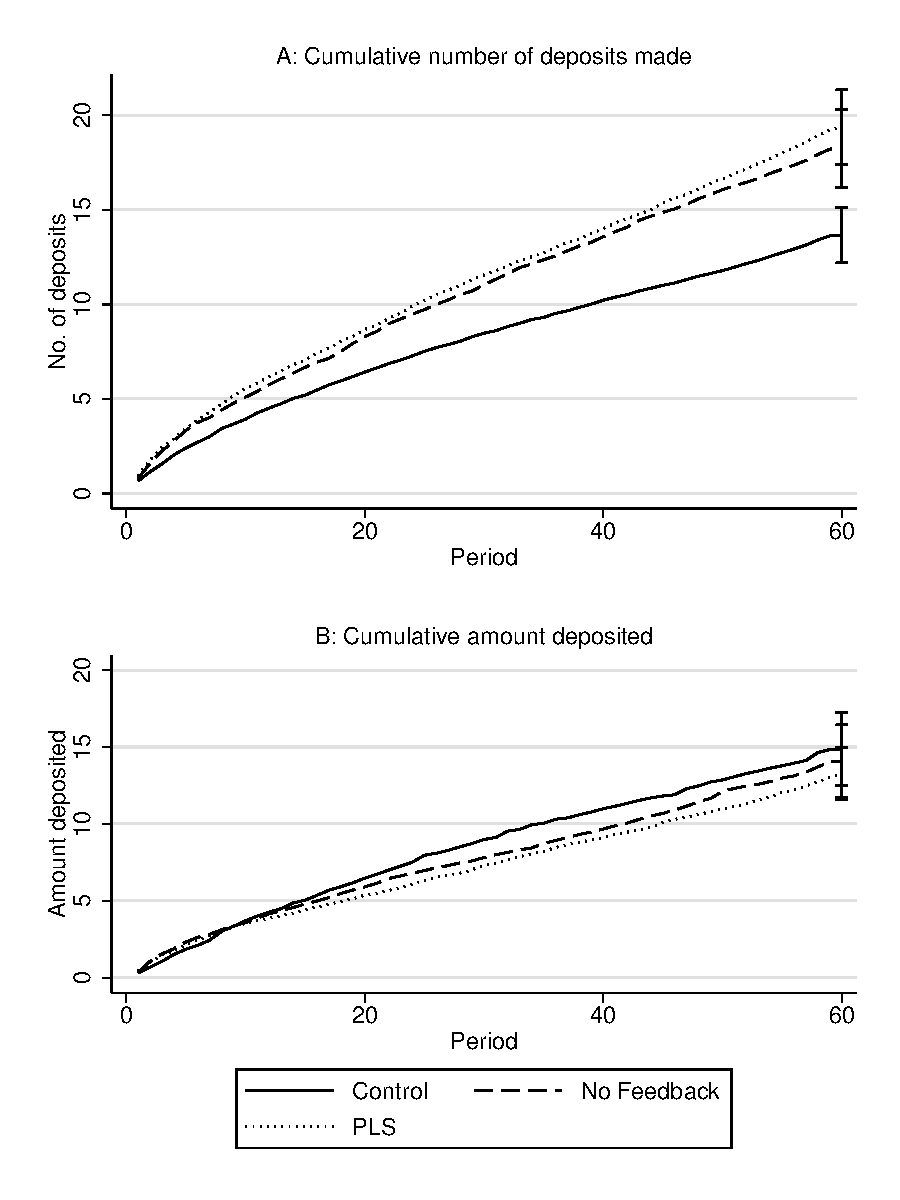
\includegraphics[height=0.85\textheight]{../../figures/line-cumdeposits.pdf}
			\label{fig:line-cumdeposits}
			\caption*{\footnotesize \emph{Notes:} Panel A plots the cumulative number of deposits made by the average participant over the 60-day savings period by treatment assignment. Panel B plots the cumulative amount deposited by the average participant. Error bars for totals by the end of the project are 95\% confidence intervals for the group means.}
		\end{figure}

		\clearpage

		While effects on number of deposits are considerable, we find no effect of either treatment on total amount deposited over the project period. Panel B of Figure \ref{fig:line-cumdeposits} plots the cumulative deposit amounts, averaged by treatment group, over the 60-day period. We cannot distinguish total deposit amounts between any of the three incentive schemes. Table \ref{tab:reg-mde} reports MDEs larger than what we estimate, suggesting a lack of statistical power and not the absence of an effect. Participants with PLS and feedback withdrew a larger amount relative to the control on average ($\hat \beta = 1.63, p < 0.05$) but we are unable to detect statistically significant differences in the final balance across treatment groups.

		\begin{table}[h]\centering \def\sym#1{\ifmmode^{#1}\else\(^{#1}\)\fi} \caption{Minimum detectable effect sizes} \label{tab:reg-mde} \maxsizebox*{\textwidth}{\textheight}{ \begin{threeparttable} \begin{tabular}{l*{3}{c}} \toprule
          &\multicolumn{1}{c}{(1)}&\multicolumn{1}{c}{(2)}&\multicolumn{1}{c}{(3)}\\
          &\multicolumn{1}{c}{Lottery MDE}&\multicolumn{1}{c}{\specialcell{Control Mean\\(SD)}}&\multicolumn{1}{c}{N}\\
\midrule
Total no. of deposits&     7.09&    13.66&      311\\
          &         &  (15.08)&         \\
No. of days saved&     5.77&    11.78&      311\\
          &         &  (12.93)&         \\
Daily avg. no. of deposits&     0.12&     0.23&      311\\
          &         &   (0.25)&         \\
Total deposit amt.&     9.38&    14.87&      311\\
          &         &  (24.48)&         \\
Total withdrawal amt.&     2.65&     1.07&      311\\
          &         &   (4.53)&         \\
Total savings last mo. (USD PPP)&    70.69&    80.31&      284\\
          &         & (112.74)&         \\
M-Pesa savings last mo. (USD PPP)&    17.80&    20.42&      284\\
          &         &  (44.67)&         \\
ROSCA savings last mo. (USD PPP)&    18.98&    22.24&      283\\
          &         &  (42.18)&         \\
Currently saves with ROSCA&     0.20&     0.54&      284\\
          &         &   (0.50)&         \\
Gamble more&     0.14&     0.12&      284\\
          &         &   (0.32)&         \\
\bottomrule \end{tabular} \begin{tablenotes}[flushleft] \footnotesize \item \emph{Notes:} Column 1 reports the minimum detectable effect sizes of the lottery treatment compared to control on the row variables with \(\alpha\) = 0.05 and 0.8 power. Columns 2 - 3 report the control group means and SDs and size of the analytic sample respectively. \end{tablenotes} \end{threeparttable} } \end{table}


		Our results are consistent with a general finding among earlier experiments on lottery-based incentives that behavioral responses occur on the extensive, but not intensive, margin. \shortciteN{brune_effect_2015} test a stochastic incentive in Malawi wherein tea harvesters entered a lottery conditional on attendance and could increase their probability of a prize according to their output. That study found significant improvements in workplace attendance persisting over 13 weeks without changes in output. \shortciteN{loibl_testing_2016}, examining features of the Individual Development Account program in the U.S., find no effect of PLS over certain returns of equal expected value. A recent experiment by \shortcite{gertler_long-term_2017} randomized the provision of PLS across banks in Mexico and observed a 43\% increase in the number of account openings in the month the lotteries were in effect but without affecting balances. Tests of PLS in the lab arrive at results slightly different from our own. \shortciteN{atalay_savings_2014} conducted an online portfolio-choice experiment in the U.S. that resulted in subjects saving an additional 12 percentage points more with prize-linked and regular savings than with regular savings alone. \shortciteN{dizon_leveraging_2016} replicate this design in an experiment conducted in Haiti and indentify a 22\% increase in savings.\footnote{\shortciteN{dizon_leveraging_2016} emphasize that savings responded to the presence of the stochastic component rather than expected returns.} In an experiment with undergraduates, \shortciteN{filiz-ozbay_lottery_2015} found that subjects are willing to accept a lower rate of return to delay a payment when the return is stochastic than when it is deterministic. Their designs differed from the present study in one important respect: subjects were provided budgets in order to make portfolio allocations. With a median monthly income of USD 77, households in our study may be too liquidity constrained to sustain a larger balance with PLS. Baseline correlations suggest that monthly income is predictive of savings in the mobile product \textit{ceteris paribus} though we do not observe heterogeneity of the treatment effect conditional on income.

		That potential savers respond to PLS by making more frequent deposits can be explained as the subdivision of lotteries to reduce risk \shortciteN{samuelson_risk_1963}.

		That potential savers respond to PLS on the extensive margin is consistent with an ``entertainment'' utility hypothesis of gambling \shortcite{conlisk_utility_1993}. That is, consumers will behave in ways that enable them to make gambles irrespective of potential earnings. Under this hypothesis, an increase in the number of deposits in the treatment group is expected if merely making a deposit on a certain day qualifies participants to play the lottery for that day. Recall that participants indeed had almost five more active days---and thus play the lottery five more times---than the control group. Unsurprisingly, participants are not making more deposits \textit{within} days since this does not affect lottery eligibility. Thus, the overall effect of the PLS is to encourage savers to make more deposits without a corresponding increase in amount saved.

		% there are three different kinds of behavioral responses here: 1) opening an account, 2) playing the lottery, and 3) putting more money into the lottery. literature finds 1) and not 3) and that can be explained by the standard theories of gambling. our study doesnt measure that because we opened accounts for everyone in the sample. likewise, i dont think they measure 2). it is entirely possible that people deposit to play more. alternatively, people save more frequently in order to reduce risk (rethink entire paper?)

			% if you introduce risk, i still sure will take the bet as long as i can subdivide in order to reduce risk because i am risk averse (this is a standard reponse, but you could only observe this in dynamic settings)
			% its not that i like gambling, its that i want positive returns (as in control group) but would rather spread it to smooth out
			% maybe people would put more money into PLS if they had it (regular gambling theories) but since they just want returns, they deposit the same as control but more often to smooth it out

		% people feel luckier, regret lottery groups select into regret (they want feedback and the lottery)
		% Do they play because of non-divisible large expenditures like \shortciteN{herskowitz__2016} http://blogs.worldbank.org/impactevaluations/unmet-liquidity-needs-and-spread-sports-betting-guest-post-sylvan-herskowitz? no savings and lottery both do that.

		% \begin{table}[ht]\centering \def\sym#1{\ifmmode^{#1}\else\(^{#1}\)\fi} \caption{Treatment effects -- Hypothetical treatment assignment} \label{tab:reg-fwerselect} \maxsizebox*{\textwidth}{\textheight}{ \begin{threeparttable} \begin{tabular}{l*{5}{c}} \toprule
          &\multicolumn{3}{c}{Effect estimates}&\multicolumn{2}{c}{Sample}\\\cmidrule(lr){2-4}\cmidrule(lr){5-6}
          &\multicolumn{1}{c}{(1)}&\multicolumn{1}{c}{(2)}&\multicolumn{1}{c}{(3)}&\multicolumn{1}{c}{(4)}&\multicolumn{1}{c}{(5)}\\
          &\multicolumn{1}{c}{No Feedback}&\multicolumn{1}{c}{PLS}&\multicolumn{1}{c}{\specialcell{PLS-\\No Feedback}}&\multicolumn{1}{c}{\specialcell{Control Mean\\(SD)}}&\multicolumn{1}{c}{Obs.}\\
\midrule
Select control group&-0.13\sym{*}&    -0.08&     0.05&     0.41&      284\\
          &   (0.07)&   (0.07)&   (0.07)&   (0.50)&         \\
          &   [0.20]&   [0.64]&   [0.90]&         &         \\
Select No Feedback group&     0.02&    -0.11&-0.13\sym{*}&     0.55&      284\\
          &   (0.07)&   (0.07)&   (0.07)&   (0.50)&         \\
          &   [1.00]&   [0.34]&   [0.24]&         &         \\
Select PLS group&0.12\sym{***}&0.19\sym{***}&     0.07&     0.03&      284\\
          &   (0.04)&   (0.05)&   (0.06)&   (0.18)&         \\
          &[0.02\sym{**}]&[0.00\sym{***}]&   [0.48]&         &         \\
Perceived effect of PLS without feedback&    -0.67&    -2.36&    -1.69&     2.27&      283\\
          &   (4.86)&   (3.44)&   (4.55)&  (26.53)&         \\
          &   [1.00]&   [0.72]&   [0.96]&         &         \\
Perceived effect of PLS&    -3.71&     0.58&     4.29&    -3.90&      283\\
          &   (7.07)&   (4.49)&   (6.56)&  (35.85)&         \\
          &   [0.96]&   [0.88]&   [0.96]&         &         \\
\bottomrule \end{tabular} \begin{tablenotes}[flushleft] \footnotesize \item \emph{Notes:} Columns 1--3 report OLS estimates of the treatment effect. Standard errors are in parentheses and FWER adjusted \(p\)-values are in brackets. Observations are at the individual level. * denotes significance at 10 pct., ** at 5 pct., and *** at 1 pct. level. Stars on the coefficient estimates reflect unadjusted \(p\)-values. \end{tablenotes} \end{threeparttable} } \end{table}

% File produced by reg-fwer.do with /Users/justin/Repos/akiba-lottery-pub/data/clean/akiba_wide.dta on 15:50:28 11 Mar 2020 by user justin on Stata 13.1 with seed X7da58e996cc9a9f9707bcb9490ad99a500041535
		% \begin{table}[ht]\centering \def\sym#1{\ifmmode^{#1}\else\(^{#1}\)\fi} \caption{Treatment effects -- Self-perceptions} \label{tab:reg-fwerself} \maxsizebox*{\textwidth}{\textheight}{ \begin{threeparttable} \begin{tabular}{l*{5}{c}} \toprule
          &\multicolumn{3}{c}{Effect estimates}&\multicolumn{2}{c}{Sample}\\\cmidrule(lr){2-4}\cmidrule(lr){5-6}
          &\multicolumn{1}{c}{(1)}&\multicolumn{1}{c}{(2)}&\multicolumn{1}{c}{(3)}&\multicolumn{1}{c}{(4)}&\multicolumn{1}{c}{(5)}\\
          &\multicolumn{1}{c}{PLS-N}&\multicolumn{1}{c}{PLS-F}&\multicolumn{1}{c}{\specialcell{PLS-F $-$ \\PLS-N}}&\multicolumn{1}{c}{\specialcell{Control Mean\\(SD)}}&\multicolumn{1}{c}{Obs.}\\
\midrule
Do you see yourself as a saver?&    -0.20&    -0.09&     0.11&    -0.00&      284\\
          &   (0.15)&   (0.14)&   (0.15)&   (1.00)&         \\
          &   [0.60]&   [1.00]&   [1.00]&         &         \\
Are you in general a lucky person?&4.77\sym{***}&4.97\sym{***}&     0.20&    -0.00&      284\\
          &   (0.20)&   (0.18)&   (0.23)&   (1.00)&         \\
          &[0.00\sym{***}]&[0.00\sym{***}]&   [0.80]&         &         \\
Do you feel you saved enough?&     0.19&    -0.09&-0.28\sym{*}&     0.00&      284\\
          &   (0.15)&   (0.15)&   (0.15)&   (1.00)&         \\
          &   [0.60]&   [1.00]&   [0.20]&         &         \\
How did you feel not saving?&    -0.02&     0.06&     0.08&    -0.00&      284\\
          &   (0.16)&   (0.15)&   (0.16)&   (1.00)&         \\
          &   [1.00]&   [1.00]&   [1.00]&         &         \\
\bottomrule \end{tabular} \begin{tablenotes}[flushleft] \footnotesize \item \emph{Notes:} Columns 1--3 report OLS estimates of the treatment effect. Standard errors are in parentheses and FWER adjusted \(p\)-values are in brackets. Observations are at the individual level. * denotes significance at 10 pct., ** at 5 pct., and *** at 1 pct. level. Stars on the coefficient estimates reflect unadjusted \(p\)-values. \end{tablenotes} \end{threeparttable} } \end{table}

% File produced by reg-fwer.do with /Users/justin/Repos/akiba-lottery-pub/data/clean/akiba_wide.dta on 11:52:03 25 Oct 2020 by user justin on Stata 13.1 with seed X27e0a1708256a41cdeaf4038df2ac2a9000400f4

	\subsection{Regret Aversion is a Potential Mechanism}

		Our estimates on the effect of \textsc{Lottery} are smaller in magnitude to the effect of \textsc{Regret} and are not significant at the 5\% level. Why might PLS with feedback elicit a larger behavioral response than PLS alone? Two alternative, but not mutually exclusive mechanisms could be driving these results. First, recall that participants in \textsc{Regret} automatically received lottery tickets at the beginning of each day while \textsc{Lottery} participants had to make deposits before obtaining a ticket. Participants who exhibit loss aversion will thus be more willing to save to prevent losing a ticket already in hand \shortcite{kahneman_advances_1992}. Second, participants save to minimize anticipated regret from winning the lottery but being unable to claim the prize. This mechanism is inactive in the PLS treatment alone because that group only receives lottery results after saving.

		\begin{figure}[ht]
		\centering
		\caption{Timing of deposits}
		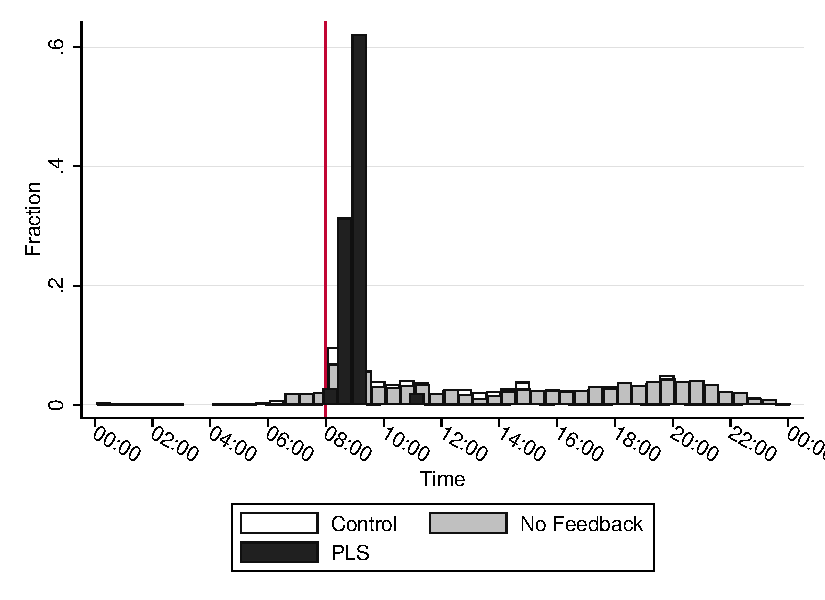
\includegraphics[width=\textwidth]{../../figures/hist-deposits.pdf}
		\label{fig:hist-deposits}
		\caption*{\footnotesize \emph{Notes:} This figure plots the empirical distribution of timing of all deposits over the project period. Each bin spans 30 minutes with a height equal to the fraction of all deposits within each treatment group. Participants received the first SMS at 8:00 that summarized how much the participant saved the previous day, how much the participant earned through a matching contribution or winnings, and their total balance. An hour later, participants received a second SMS encouraging them to save that day. Participants in \textsc{Regret} received a new lottery ticket with the second message.}
		\end{figure}

		We estimate Equation \ref{eq:regret} to test for the presence of regret aversion distinct from other potential channels. Under the regret aversion hypothesis, we expect to observe an additional effect on saving after participants receive feedback on a winning ticket rather than a losing ticket. Table \ref{tab:reg-regretaversion} shows that \textsc{Regret} participants are 2 percentage points ($p<0.05$) more likely to make a deposit after learning about a winning ticket. This effect is small but is statistically distinguishable from the group's average effect. The portion of the treatment effect arising from other mechanisms is significant at the 5\% level so we are unable to rule them out using this test. Figure \ref{fig:hist-deposits} plots the distribution of deposits over time and shows timing suggestive of regret aversion. Nearly all deposits made in the \textsc{Regret} group ocurred within an hour of announcing the lottery results from the previous day. Deposits similarly peaked between the results and the disbursement of that day's lottery ticket. We observe no similar pattern in the \textsc{Lottery} and control groups.

		\begin{table}[ht]\centering \def\sym#1{\ifmmode^{#1}\else\(^{#1}\)\fi} \caption{Regression of deposits on lottery results} \label{tab:reg-regretaversion} \maxsizebox*{\textwidth}{\textheight}{ \begin{threeparttable} \begin{tabular}{l*{2}{c}} \toprule
                &\multicolumn{1}{c}{Made a deposit}\\
\midrule
Winning ticket  &     0.02\sym{**} \\
                &   (0.01)         \\
\midrule
Adjusted \(R^{2}\)&    0.081         \\
Control mean    &     0.20         \\
Daily PLS effect&                  \\
Observations    &     4473         \\
\bottomrule \end{tabular} \begin{tablenotes}[flushleft] \footnotesize \item \emph{Notes:} This table reports on a regression of having saved at period \(t\) on winning the lottery at \(t\) conditional on being in the PLS group and not having saved at \(t-1\). The unit of observation is individual-by-period. The regression includes period fixed effects. Standard errors are in parentheses and clustered at the individual level. * denotes significance at 10 pct., ** at 5 pct., and *** at 1 pct. level. \end{tablenotes} \end{threeparttable} } \end{table}

% File produced by akiba-estimate.do with /Users/justin/Repos/akiba-lottery-pub/data/clean/akiba_long.dta on 11:52:17 25 Oct 2020 by user justin on Stata 13.1 with seed Xd950c82044e7d5a124b5a3e57a7d26c000042a30

		\clearpage

	% \subsection{Effect on Deposits Persists Over Time}

		% we do not find evidence that this decreases (except afte rthe first few days)
		% this has been documented in the lab with small stakes and repeated decisions. erev demonstrates that people who take median 15 (weber 2007 17) with replacement are less likely to overweight rare events. also erev speculates that this is through experience with the rare event and demonstrates it. alternatively, overweighting of recent evidence. does winning affect decision to play in this study?

		% bilal zia paper on debiasing

		% \begin{table}[h]\centering \def\sym#1{\ifmmode^{#1}\else\(^{#1}\)\fi} \caption{Treatment effects conditional on days elapsed} \label{tab:reg-timetrend} \maxsizebox*{\textwidth}{\textheight}{ \begin{threeparttable} \begin{tabular}{l*{2}{c}} \toprule
                &\multicolumn{1}{c}{(1)}&\multicolumn{1}{c}{(2)}\\
                &\multicolumn{1}{c}{No. of deposits made}&\multicolumn{1}{c}{Amount deposited (USD PPP)}\\
\midrule
Lottery         &    0.109\sym{**} &   -0.044         \\
                &  (0.052)         &  (0.085)         \\
Regret          &    0.116\sym{**} &   -0.074         \\
                &  (0.051)         &  (0.076)         \\
Savings period  &   -0.004\sym{***}&   -0.003\sym{**} \\
                &  (0.001)         &  (0.001)         \\
Lottery $\times$ Savings period&   -0.001         &    0.001         \\
                &  (0.001)         &  (0.002)         \\
Regret $\times$ Savings period&   -0.001         &    0.002         \\
                &  (0.001)         &  (0.002)         \\
Constant        &    0.351\sym{***}&    0.351\sym{***}\\
                &  (0.033)         &  (0.070)         \\
\midrule
Adjusted \(R^{2}\)&    0.026         &    0.003         \\
Lottery $\times$ period = Regret $\times$ period \(p\)-value&    0.682         &    0.607         \\
Observations    &    18636         &    18636         \\
\bottomrule \end{tabular} \begin{tablenotes}[flushleft] \footnotesize \item \emph{Notes:} This table reports a regression of savings activity on treatment indicators and a linear time trend. The unit of observation is individual-period. Standard errors are in parentheses and clustered at the individual level. * denotes significance at 10 pct., ** at 5 pct., and *** at 1 pct. level. \end{tablenotes} \end{threeparttable} } \end{table}

% File produced by akiba-estimate.do with /n/homeserver2/user2a/justinra/repos/akiba-lottery-pub/data/clean/akiba_long.dta on 07:40:40 15 Feb 2018 by user justinra on Stata 13.1 with seed Xf05030d3966aec1c00305ad5d96d12ae00042416
		% add effects over time
		%
		% \begin{figure}[ht]
		% \caption{Effects over time -- Number of deposits}
		% 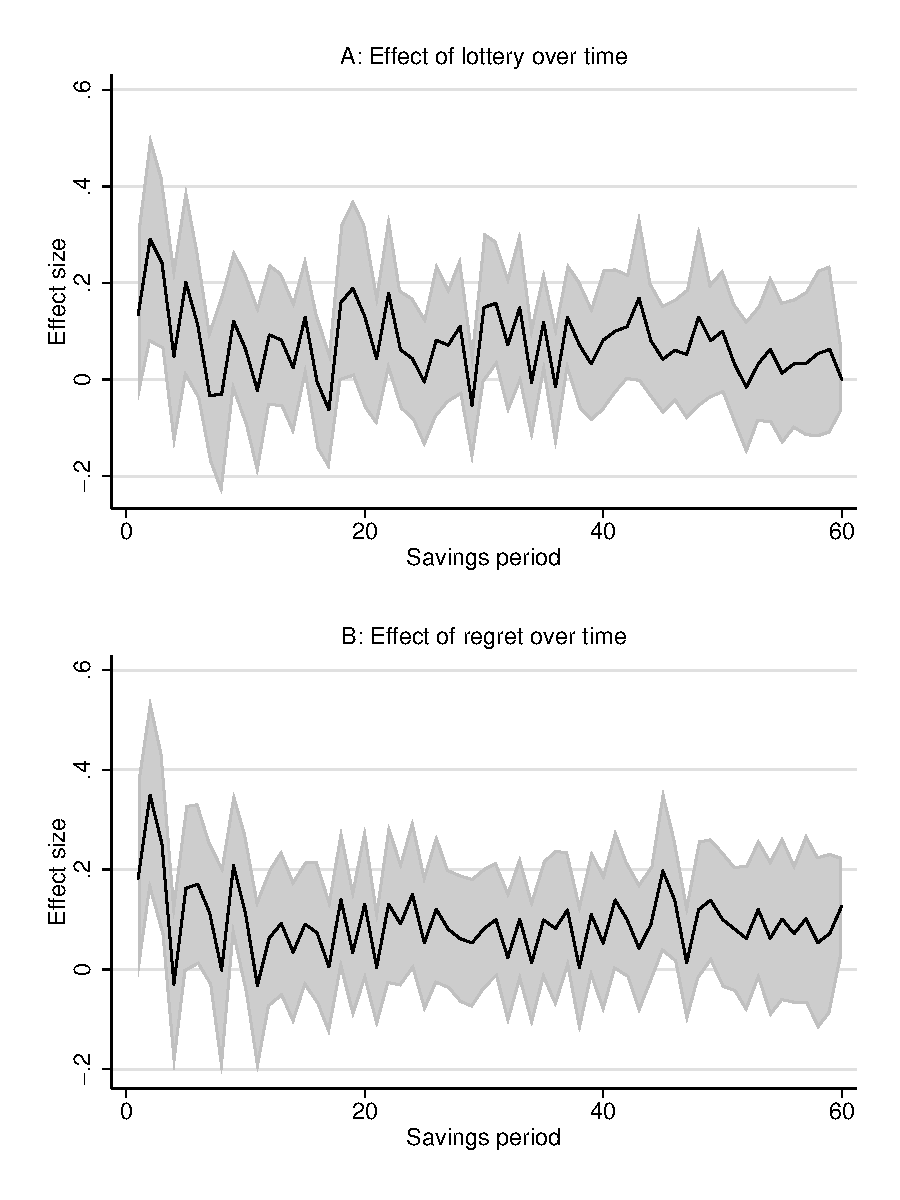
\includegraphics[width=\textwidth]{../../figures/line-timemobile_deposits.pdf}
		% \caption*{\footnotesize \emph{Notes:} Panel A plots the treatment effect of \textsc{Lottery} on number of deposits as a function of savings period. Panel B plots the treatment effect of \textsc{Regret} on number of deposits as a function of savings period. Shaded areas represent 95\% confidence regions.}
		% \end{figure}

		% \begin{figure}[ht]
		% \caption{Effects over time -- Amount deposited}
		% 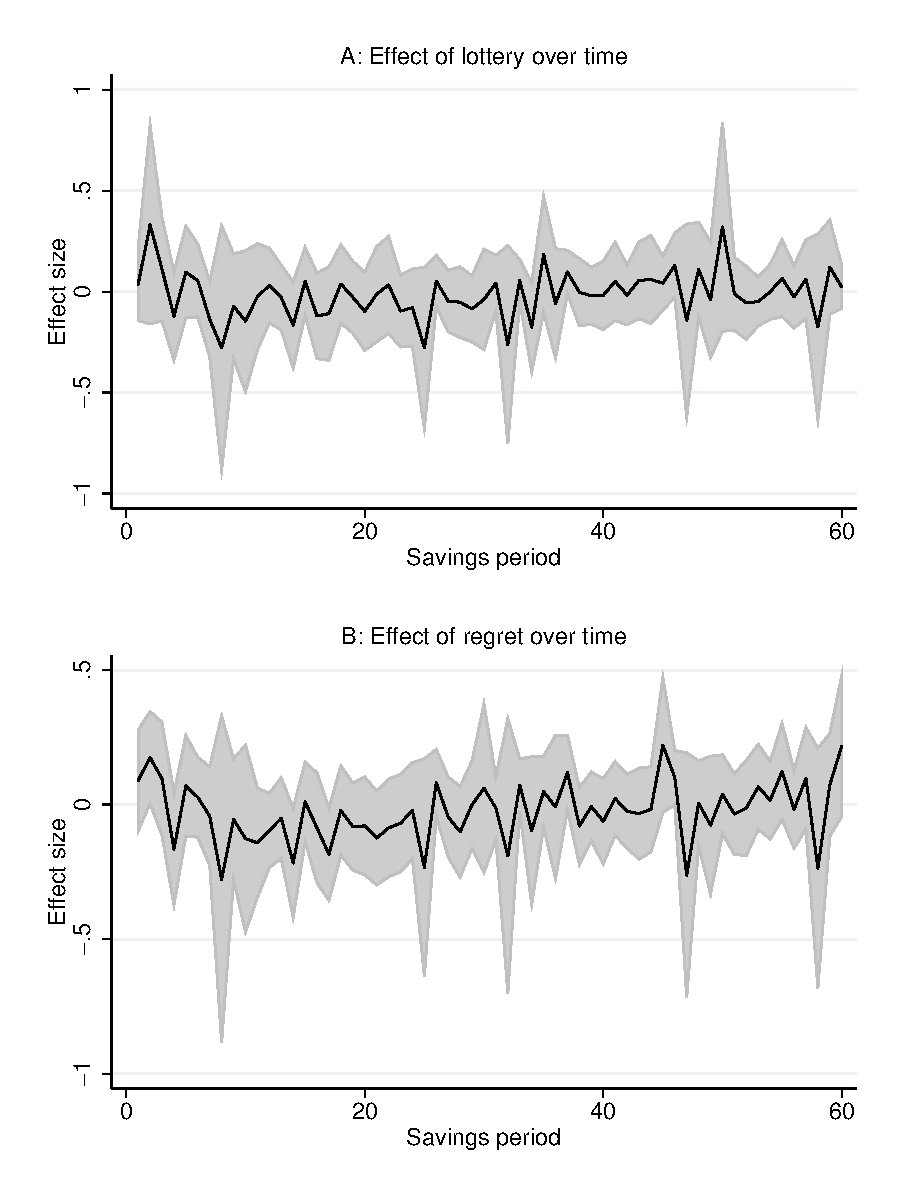
\includegraphics[width=\textwidth]{../../figures/line-timemobile_depositamount.pdf}
		% \caption*{\footnotesize \emph{Notes:} Panel A plots the treatment effect of \textsc{Lottery} on amount deposited as a function of savings period. Panel B plots the treatment effect of \textsc{Regret} on amount deposited as a function of savings period. Shaded areas represent 95\% confidence regions.}
		% \end{figure}

	\subsection{PLS with Feedback Encourages Particpation in Informal Saving}

		A related objective of this study is to examine whether PLS act as complements or substitutes to existing savings products. We do not find evidence that PLS crowds out saving by other means. Table \ref{tab:reg-fwersave} reports no statistically significant effect on total saving through M-Pesa or ROSCAs. We do find, however, that respondents in \textsc{Regret} are 14 percentage points ($p < 0.05$) more likely to save with a ROSCA compared to the control group and 16 percentage points ($p < 0.05$) more likely relative to \textsc{Lottery}. This result is robust to the inclusion of covariates but is not significant when correcting for multiple inference ($p < 0.1$). We find no effect of \textsc{Lottery} on informal saving. Table \ref{tab:het-labor_employed_0} reports heterogeneous treatment effects on our primary outcomes by employment status. Column 3 shows that the segment of our sample who are unemployed drive the effect on ROSCA participation. Overall, we do not find that PLS cannibalizes savings from other sources.

		% is this consistent with results?
		% \shortciteN{shawn_allen_cole_can_2014} and \shortciteN{dizon_leveraging_2016} + experimental guys + gertler

		\begin{table}[ht]\centering \def\sym#1{\ifmmode^{#1}\else\(^{#1}\)\fi} \caption{Treatment effects -- Savings outside the project} \label{tab:reg-fwersave} \maxsizebox*{\textwidth}{\textheight}{ \begin{threeparttable} \begin{tabular}{l*{5}{c}} \toprule
          &\multicolumn{3}{c}{Effect estimates}&\multicolumn{2}{c}{Sample}\\\cmidrule(lr){2-4}\cmidrule(lr){5-6}
          &\multicolumn{1}{c}{(1)}&\multicolumn{1}{c}{(2)}&\multicolumn{1}{c}{(3)}&\multicolumn{1}{c}{(4)}&\multicolumn{1}{c}{(5)}\\
          &\multicolumn{1}{c}{Lottery}&\multicolumn{1}{c}{Regret}&\multicolumn{1}{c}{\specialcell{Regret-\\Lottery}}&\multicolumn{1}{c}{\specialcell{Control Mean\\(SD)}}&\multicolumn{1}{c}{Obs.}\\
\midrule
Total savings last month&    18.45&   -17.87&   -36.32&    80.31&      284\\
          &  (25.16)&  (14.64)&  (24.06)& (112.74)&         \\
          &   [1.00]&   [1.00]&   [0.20]&         &         \\
M-Pesa savings last month&    -5.42&    -6.71&    -1.29&    20.42&      284\\
          &   (6.34)&   (5.49)&   (5.30)&  (44.67)&         \\
          &   [1.00]&   [1.00]&   [1.00]&         &         \\
ROSCA savings last month&     1.48&     7.37&     5.89&    22.24&      283\\
          &   (6.76)&   (6.79)&   (7.33)&  (42.18)&         \\
          &   [1.00]&   [1.00]&   [0.40]&         &         \\
Saves with a ROSCA&    -0.02&0.14\sym{**}&0.16\sym{**}&     0.54&      284\\
          &   (0.07)&   (0.07)&   (0.07)&   (0.50)&         \\
          &   [1.00]&   [0.40]&[0.00\sym{***}]&         &         \\
\bottomrule \end{tabular} \begin{tablenotes}[flushleft] \footnotesize \item \emph{Notes:} Columns 1--3 report OLS estimates of the treatment effect. Standard errors are in parentheses and FWER adjusted \(p\)-values are in brackets. Observations are at the individual level. * denotes significance at 10 pct., ** at 5 pct., and *** at 1 pct. level. Stars on the coefficient estimates reflect unadjusted \(p\)-values. \end{tablenotes} \end{threeparttable} } \end{table}

% File produced by reg-fwer.do with /Users/justin/Repos/akiba-lottery-pub/data/clean/akiba_wide.dta on 00:15:52 13 Jun 2019 by user justin on Stata 13.1 with seed X27e0a1708256a41cdeaf4038df2ac2a9000400f4
		\begin{table}[htbp]\centering \def\sym#1{\ifmmode^{#1}\else\(^{#1}\)\fi} \caption{Heterogeneous effects - Primary outcomes by employed} \label{tab:het-labor_employed_0} \maxsizebox*{\paperwidth}{\paperheight}{ \begin{threeparttable} \begin{tabular}{l*{4}{c}} \toprule
                &\multicolumn{1}{c}{(1)}&\multicolumn{1}{c}{(2)}&\multicolumn{1}{c}{(3)}&\multicolumn{1}{c}{(4)}\\
                &\multicolumn{1}{c}{Total no. of deposits}&\multicolumn{1}{c}{Avg. no. of deposits}&\multicolumn{1}{c}{No. of days saved}&\multicolumn{1}{c}{Gamble more}\\
\midrule
Lottery         &     4.67         &     0.02         &     3.18         &     0.17\sym{**} \\
                &   (3.69)         &   (0.06)         &   (2.67)         &   (0.07)         \\
Lottery $\times$ \\ Employed&    -0.56         &    -0.09         &     1.01         &    -0.21\sym{**} \\
                &   (5.11)         &   (0.08)         &   (4.07)         &   (0.10)         \\
Regret          &     9.02\sym{***}&    -0.04         &     7.96\sym{***}&     0.17\sym{***}\\
                &   (3.28)         &   (0.04)         &   (2.78)         &   (0.07)         \\
Regret $\times$ \\ Employed&    -6.82         &     0.05         &    -6.22         &    -0.04         \\
                &   (4.91)         &   (0.08)         &   (4.18)         &   (0.11)         \\
Employed        &     4.53         &     0.01         &     4.13         &     0.14\sym{**} \\
                &   (2.93)         &   (0.06)         &   (2.51)         &   (0.06)         \\
Constant        &    11.42\sym{***}&     1.15\sym{***}&     9.74\sym{***}&     0.04         \\
                &   (1.76)         &   (0.04)         &   (1.52)         &   (0.03)         \\
\midrule
Adjusted \(R^{2}\)&    0.011         &   -0.005         &    0.019         &    0.026         \\
Control mean    &    13.66         &     1.16         &    11.78         &     0.12         \\
Lottery \emph{p}-value&     0.25         &     0.24         &     0.17         &     0.63         \\
Regret \emph{p}-value&     0.55         &     0.87         &     0.58         &     0.15         \\
Observations    &      311         &      275         &      311         &      284         \\
\bottomrule \end{tabular} \begin{tablenotes}[flushleft] \footnotesize \item \emph{Notes:} This table reports OLS estimates of the treatment effect and its interaction with baseline. Standard errors are in parentheses. * denotes significance at 10 pct., ** at 5 pct., and *** at 1 pct. level. We also report the \(p\)-values for joint tests on the direct treatment effect conditional on the baseline covariate $= 1$. \end{tablenotes} \end{threeparttable} } \end{table}

% File produced by akiba_estimate.do with /Users/Justin/Repos/akiba-lottery-pub/data/clean/akiba_wide.dta on 12:20:24  2 Mar 2017 by user Justin on Stata 13.1 with seed Xf2613771df2fc417d7ddd109f297573500041f43

	\subsection{PLS with Feedback Increases Outside Gambling Behavior}

		The study asks whether PLS act as complement or substitute to existing gambling activity. At endline, we ask participants whether participants gambled more than they usually do apart from participating in the savings program. As reported in Table \ref{tab:reg-fwergamble}, we find that participants in the \textsc{Regret} group self-report higher gambling behavior the savings program. On average, treated participants are 15 percentage points ($p < 0.05$) more likely to report gambling than the control group. This finding is robust to covariate ajdustment and is significant at the 10\% level after FWER adjustment. We find no average effects for participants in the \textsc{Lottery} group but Table \ref{tab:het-labor_employed_0} shows that \textsc{Lottery} induces increased gambling among the unemployed ($\hat beta = 0.17, p < 0.05$). Our measure for gambling activity is susceptible to experimenter demand though it is unclear in what direction this might bias our estimate. With this caveat in mind, the effect provides some evidence of a complementary relationship between PLS and broader gambling behavior.

		\shortciteN{cookson_when_2016} offered individuals in Nebraska access to an PLS and observed cash withdrawals at casinos as a measure of gambling behavior. They find reductions in transactions between 7-15\% accredit the effect to attribute-based substition of casino gambling with the PLS. One important difference in the savings program from the present study is the bundling of the account with an anti-gambling campaign. Such a feature may have counteracted external gambling associated with the PLS and could explain the difference in our findings.

		% \shortciteN{shawn_allen_cole_can_2014} and \shortciteN{dizon_leveraging_2016} also find reductions in gambling

		\begin{table}[h]\centering \def\sym#1{\ifmmode^{#1}\else\(^{#1}\)\fi} \caption{Treatment effects controlling the FWER -- Gambling} \label{tab:reg-fwergamble} \maxsizebox*{\textwidth}{\textheight}{ \begin{threeparttable} \begin{tabular}{l*{5}{c}} \toprule
          &\multicolumn{3}{c}{Effect estimates}&\multicolumn{2}{c}{Sample}\\\cmidrule(lr){2-4}\cmidrule(lr){5-6}
          &\multicolumn{1}{c}{(1)}&\multicolumn{1}{c}{(2)}&\multicolumn{1}{c}{(3)}&\multicolumn{1}{c}{(4)}&\multicolumn{1}{c}{(5)}\\
          &\multicolumn{1}{c}{Lottery}&\multicolumn{1}{c}{Regret}&\multicolumn{1}{c}{\specialcell{Difference\\\(p\)-value}}&\multicolumn{1}{c}{\specialcell{Control Mean\\(SD)}}&\multicolumn{1}{c}{Obs.}\\
\midrule
Gamble more&     0.06&0.15$^{***}$&     0.16&     0.12&      284\\
          &   (0.05)&   (0.06)&         &   (0.32)&         \\
          &   [0.61]&[0.05]$^{*}$&         &         &         \\
Gamble less&    -0.02&     0.04&     0.24&     0.16&      284\\
          &   (0.05)&   (0.06)&         &   (0.37)&         \\
          &   [0.88]&   [0.80]&         &         &         \\
More tempted to gamble&     0.09&     0.05&     0.56&     0.47&      284\\
          &   (0.07)&   (0.07)&         &   (0.50)&         \\
          &   [0.61]&   [0.80]&         &         &         \\
Less tempted to gamble&    -0.01&     0.03&     0.27&     0.06&      284\\
          &   (0.03)&   (0.04)&         &   (0.25)&         \\
          &   [0.88]&   [0.80]&         &         &         \\
\bottomrule \end{tabular} \begin{tablenotes}[flushleft] \footnotesize \item \emph{Notes:} Columns 1--2 report OLS estimates of the treatment effect. Column 3 reports the \(p\)-values for tests of the equality of the two treatment effects. Standard errors are in parentheses and FWER adjusted \(p\)-values are in brackets. Observations are at the individual level. * denotes significance at 10 pct., ** at 5 pct., and *** at 1 pct. level. Stars on the coefficient estimates reflect unadjusted \(p\)-values. \end{tablenotes} \end{threeparttable} } \end{table}

% File produced by reg-fwer.do with /n/homeserver2/user2a/justinra/repos/akiba-lottery-pub/data/clean/akiba_wide.dta on 02:33:07 16 Feb 2018 by user justinra on Stata 13.1 with seed X71d1d353b37e281e006fa26738e26f4500044a1c

\section{Conclusion} \label{sec:conclusion}

		By taking advantage of savers' preference for gambling, stochastic incentive schemes like PLS represent a promising policy tool to overcome behavioral barriers to saving. We conducted a randomized experiment testing a PLS product with informal residents in Nairobi, Kenya. Utilizing a mobile savings platform, we randomly assign respondents to a savings account with a certain, matching incentive, a lottery incentive, and a lottery incentive with feedback on ex post potential lottery winnings. We set the fixed match equivalent in expectation to the lottery prize so that comparing he two groups identifies the effect of stochastic incentives compared to deterministic incentives holding amount constant. After observing account transactions over a 60-day savings period, we find that participants in the \textsc{Regret} group made between 5-6 more deposit transactions than the matched payments group without a corresponding increase in amount saved. These results suggest that savers are making more deposits in order to ``play'' and experience a non-pecuniary benefit from the lottery. We further find that participants in the \textsc{Regret} group are more likely to report increased gambling after the the end of the savings program.

		If PLS increase deposits but are ineffective at increasing a key outcome like savings, are they still useful from a policy perspective? If playing the lottery is appealing to potential savers, PLS may be able to attract new savers to open  accounts. PLS can also improve utilization among existing account holders. Frequent deposits may have long-term benefits by encouraging the formation of a savings habit \shortcite{alessie_saving_2009}. Compared to a fixed match, lottery incentives may not be revenue neutral if financial institutions incur greater transaction costs as a result of more frequent deposits. If PLS contribute to problem gambling, the program is potentially welfare-decreasing for poor households already susceptible to costly gambling behavior. Additional program components, like an anti-gambling campaign, could diminish adverse effects on outside gambling. Overall, we document important differences between PLS and fixed-incentive schemes when it comes to encouraging savings and show that product design is crucial in determining welfare implications.

		% \shortcite{gertler_long-term_2017}: We observe the opposite: although initially lower, the savings balances of  compliers  who open accounts in response to the incentive catch up to the savings balances of those who open accounts in control branches. The levels of active use of the account are similar across lottery month account openers in treatment and control branches.
		% Focus on a potentially important outcome (no. of deposits/streak) determining long-term savings behavior previously neglected in the literature (Less than 20\% of banked adults in Sub-Saharan Africa make more than 2 deposits in a month \shortcite{demirguc-kunt_global_2015})
		% This may be an effective tool to encourage savings on the _extensive_ margin
		% brune's point about temporary vs persistent preferences implications for policy
		% Can we target better? Working poor, emerging middle class, the present study's het effects
		% Effects on downstream outcomes (consumption, etc.)
		% Tighter accounting to track savings and expenditure
		% We didn't really ask about savings goals
		% Should have incorporated higher order risk preferences (CPT)
		% Would have been good to analyze how intensity of regret aversion affects the decision to save (can't because ticket generation suffers from selection)
        % Might want to test variation in skewness holding spread constant
		% Our results target a specific behavior: people who have savings account but don't use them
		% demand is strong (tufano/cole) but actually people don't save more (it doesnt meet policy goals exactly) (it is not straightforward to justify PLS as a policy tool on the basis of demand)

\newpage

\bibliographystyle{achicago}
\bibliography{Lottery.bib}

% Overview of results:
%
% 	x Regret increases number of deposits (days and more per day in extensive margin) (FWER at 10%) (robust to controls)
% 	x Lottery shows some evidence but perhaps underpowered (10% FWER not)
% 	x No effect on balance
%   x Regret people withdraw more when given opportunity
%
%   x The effect occurs right after the lottery results are announced, and alot after receiving the ticket.
%   x We can't rule out endowment effect but regret aversion is still driving results.
%
% 	Lottery/Regret increases lucky person: hot hands, actually might make subjective bias worse
% 	Lottery/Regret increases self-selection into regret group: evidence of consumer demand from behavior _and_ self-report, but no desire to continue program and didn't tell friends or family
%
%   x It doesn't cannibalize other savings
% 	x Regret increases savings and usage of ROSCA
%	x Het: ROSCA effects among unemployed and unselfemployed, nothing else
%
% 	x Regret increases self-reported gambling: could be internal or external but can't distinguish, can we conclude that it doesn't displace it?
% 	x Het: gambling effects among employed, nothing else
%
% 	Effect on deposits don't change over time
%   x Effect conditional on winning but not saving (evidence of regret aversion over endowment effect)

% Possible explanations for results:
%
%	Nothing weird going on here: people don't save more because they don't like risk or skewness, they don't just not play because they like gambling, deposits increase due to liquidity constraints or spreading risk
% 	Overweighting of probabilities (no because there would have been an effect on amounts)
% 	Law (not fallacy) of large numbers (subjects are trying to spread risk)
% 	Benartzi Thaler: myopic loss aversion (?)
% 	Liquidity constraints (plausible but check structure of income)
% 	Lumpy gambling utility (plausible but how do we distinguish from others?)
% 	Usage diminishes learning curve, improves trust, etc. (can this be tested?)
% 	Why only ROSCA and not formal savings? Availability
% 	Differences in project period
% 	A possible mechanism underlying this effect could be that participating in the savings lottery affects perceived probabilities of gambling. Recall that our lottery incentive was designed so that savers faced no losses to their deposits. The experience of
% 	Table \ref{tab:reg-fwerself} shows that treated participants rate themselves as being lucky nearly 4.77 - 4.97 SDs ($p < 0.01$) higher than the control group.
%
% Our contributions:
%
% 	One of the first causal evidence of PLS on savings and gambling
% 	Developing country setting
% 	Mobile savings allow tight tracking of savings behavior
% 	Multi-period panel setting gives us dynamic information (Samuelson)
% 	Test the influence of regret aversion
% 	Focus on a potentially important outcome (no. of deposits/streak) determining long-term savings behavior previously neglected in the literature (Less than 20\% of banked adults in Sub-Saharan Africa make more than 2 deposits in a month \shortcite{demirguc-kunt_global_2015})
% 	The effect of PLS remains unclear, so we help understand through what channels PLS affects what
%
% Notes:
%
% 	no matter how much we dig into panel, a qje paper is not coming out because of our results, more refined story rather than extra analysis
% 	its promising as a great example of a null result, what are some theories about why this didnt work? i mean its a huge match so we set ourselves up for failure, theres already a ceiling effect
% 	MA: survey experiment prior duke MBA students get theory from this, lotteries work well when the interest rate is low but not as it increases
% 	think about intertemporal consumer behavior; what does it predict?; what do our results say about the prevailing model?
%
% To do:
%
% 	Go through paper comments
% 	Finish reading the Brune paper
% 	Finish reading the Gertler paper
% 	Finish reading the Zia paper
% 	Tighten discussion around main points and strong results
% 	Clean up results presentation
% 	Clean up theory section?
% 	Table with differences with PAP
% 	Update appendix with things we specified in the PAP
% 	Fix citations

\end{document}
